\documentclass[a4paper, 12pt]{article}
\usepackage[portuguese]{babel}
\usepackage[utf8]{inputenc}
\usepackage[T1]{fontenc}
\usepackage{amssymb}
\usepackage{indentfirst}
\usepackage{graphicx}
\usepackage{fancyhdr}
\usepackage{circuitikz}
\usepackage{tikz}
\usepackage{float}
\usepackage{authblk}
\usepackage{geometry}
\usepackage[colorinlistoftodos]{todonotes}
\usepackage{caption}
\geometry{a4paper, total={170mm,257mm}, left=25mm, top=25mm, right=25mm, bottom=25mm}
\usetikzlibrary{positioning}
\DeclareGraphicsExtensions{.pdf,.png,.jpg}
\makeindex
\author[]{Renato Nobre - 150146698}
\affil[]{Sistemas de Informação\\Universidade de Brasília}
\title{Trabalho 3\\Concepção do SI}
\date{16 de Novembro de 2016}
\pagestyle{fancy}
\fancyhf{}
\lhead{Descrição do SI}
\rhead{Universidade de Brasília\\IE - Departamento de Ciência da Computação}
\headsep = 40pt
\captionsetup{labelformat=empty}
\begin{document}
	\begin{titlepage}

		\newcommand{\HRule}{\rule{\linewidth}{0.5mm}}
		\centering
        %\maketitle
	    \textsc{\LARGE Universidade de Brasília}\\[0.5cm]
	    
\includegraphics{logo.jpg}\\[0.5cm]
		\textsc{\Large Instituto de Ciências Exatas}\\[0.5cm]
	    \textsc{\Large Departamento de Ciência da Computação}\\[0.5cm]
		\textsc{\Large Sistemas de Informação}\\[0.5cm]
	    \HRule \\[0.2cm]
	    { \huge \bfseries Trabalho 3\\[0.5cm] Concepção do SI}\\
	      \HRule \\[1.5cm]
	      	\begin{minipage}{0.4\textwidth}
	      		\begin{flushleft} \large
	      			\emph{Nome:}\\
					\emph{Renato Nobre}\\
	      		\end{flushleft}
	      	\end{minipage}
	      	~
	      	\begin{minipage}{0.4\textwidth}
	      		\begin{flushright} \large
	      			\emph{Matrícula:}\\
	       			\textsc{15/0146698}\\
	      		\end{flushright}
	      	\end{minipage}\\[8.5cm]
		\textsc{\large \centering 16 de Novembro de 2016}\\
	\end{titlepage}


	\section{Visão Geral}


    \noindent \\\textbf{Visão Geral para o Projeto HazeTasks}\\
    
    \noindent Versão 1.0\\
    
    \noindent Visão:\\
    
    A troca de tarefas entre os setores da empresa HazeApps não é bem desenvolvida, os chefes de desenvolvimento, desenvolvedores e artistas não distribuem devidamente seus afazeres. Portanto a empresa decidiu aplicar um sistema de informação para realizar a troca de tarefas.

    Ao abrir o SI, irá aparecer uma tela de login. Na tela de login haverá uma opção, novo cadastro, está opção direcionará o usuário a uma nova tela onde irá disponibilizar seu usuário, senha e cargo. Após a usuário se cadastrar ele será redirecionado novamente para tela de login. O usuário terá acesso ao quadro de tarefas de arte onde ele pode criar novas tarefas, editar tarefas em andamento e marcar tarefas já concluídas. 
    
    O sistema deve permitir que um usuário produza relatório das tarefas concluídas, bem como das tarefas em andamento. \\

    \noindent Restrições:\\ 

    • O SI não permite marcações detalhadas como \textit{labels} e atribuições.\\
    
    • A interface é extremamente básica.\\
    
	\section{Casos de Uso}
	
	\subsection{Casos de Uso Geral}
	
	\begin{figure}[H]
		\centering
		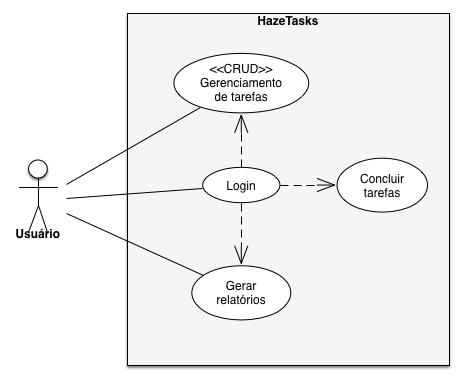
\includegraphics[scale=0.6]{usecase.png}
		\caption{Casos de Uso Geral}
	\end{figure}
	
	\subsection{Casos de Uso Extendido}
	
	\noindent \\\textbf{Caso de Uso: <<CRUD>> Gerenciamento de tarefas}
	
	1. O usuário escolhe a operação:
	
	1. Nova tarefa
	
	2. Editar Tarefa
	
	3. Consultar detalhes da tarefa
	
	4. Concluir Tarefa\\
	\textbf{Variante 1.1: Nova tarefa}\\
	1.1.1 O usuário informa: nome da tarefa, descrição, e data\\
	\textbf{Variante 1.2: Editar tarefa}\\
	1.2.1 O sistema informa todos os dados atuais da tarefa e fornece a opção de qual deseja editar\\
	1.2.2 O usuário escolhe qual informação quer editar\\
	1.2.3 O usuário pode nesta seção excluir a tarefa (tarefas excluídas não serão disponibilizadas em relatórios) \\
	\textbf{Variante 1.3: Consultar detalhes da tarefa}\\
	1.3.1 O usuário escolhe uma tarefa a qual deseja saber mais\\
	1.3.2 O sistema mostra os detalhes desta tarefa\\
	\textbf{Variante 1.4: Concluir tarefa}\\
	1.4.1 O usuário marca a tarefa escolhida como concluída\\
	
	\section{Diagrama de Raias}
	
	O diagrama de atividades, ou diagrama de raias, elabora abaixo, representa a atividade padrão do HazeTasks em uma abordagem geral. Ele demonstra o processo de gerenciamento de tarefas, desde o login até o encerramento das atividades. Como o SI e OAS, sistema de automação de escritório, não há necessidade de comunicação com órgãos externos a empresa, isto é facilmente identificável pela presença de apenas duas raias no modelo.
	
	\begin{figure}[H]
		\centering
		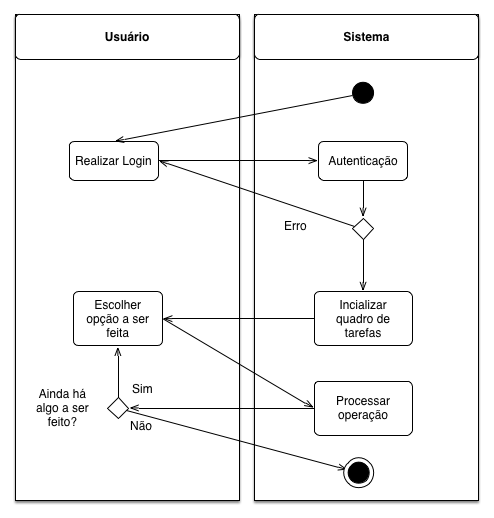
\includegraphics[scale=0.6]{actvdiagram.png}
		\caption{Diagrama de Raias}
	\end{figure}
	
	\newpage
	
	\section{Máquina de Estados}
	
	A máquina de estados do HazeTasks mostra de maneira simplificada os possíveis estados do sistema de informação. Um pequeno detalhe omitido do diagrama para facilitar o entendimento é que após os 4 estados de tarefa é possível voltar para o estado de opção escolhida e realizar outra tarefa diferente. É possível também, mostrar relatórios no momento em que desejar.\\\\
	
	\begin{figure}[H]
		\centering
		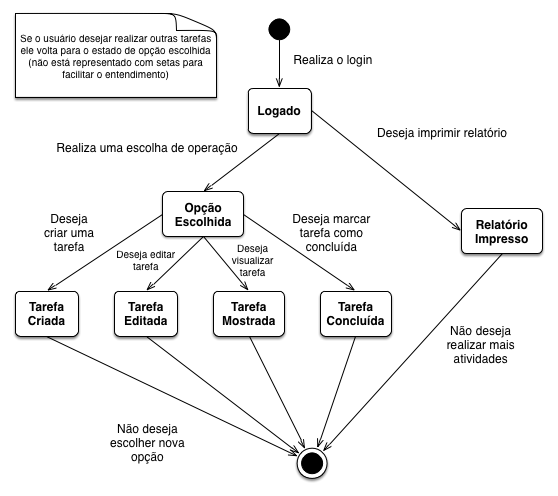
\includegraphics[scale=0.6]{statemachine.png}
		\caption{Máquina de Estados}
	\end{figure}
	
	\newpage
	
	\section{Sequencia de Eventos}
	
	O SI descrito possui poucos eventos sequenciais. De fato, a única tarefa necessária e suficiente para a realização das outras é o login. Todos os outros eventos podem ser realizados de maneira independente, exceto obviamente quando não existe nenhuma tarefa para modificar, visualizar, marcar como concluída ou imprimir relatórios. \\\\
	
	\begin{figure}[H]
		\centering
		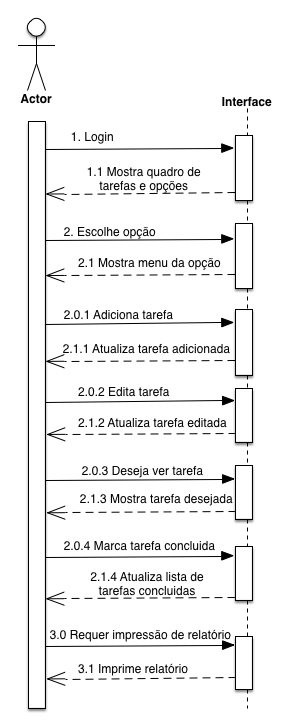
\includegraphics[scale=0.6]{eventsequence.png}
		\caption{Sequencia de Eventos}
	\end{figure}
	
	\newpage
	
	\section{Cronograma de Execução}
	
	O cronograma de execução foi feito com base no tempo disponível, tentando executar o máximo possível sem estender muito a duração do trabalho, sobrando assim, tempo para realização de atividades de outras matérias. No calendário abaixo o cronograma de execução para o trabalho de SI está representado pela cor marrom.\\\\
	
	\begin{figure}[H]
		\centering
		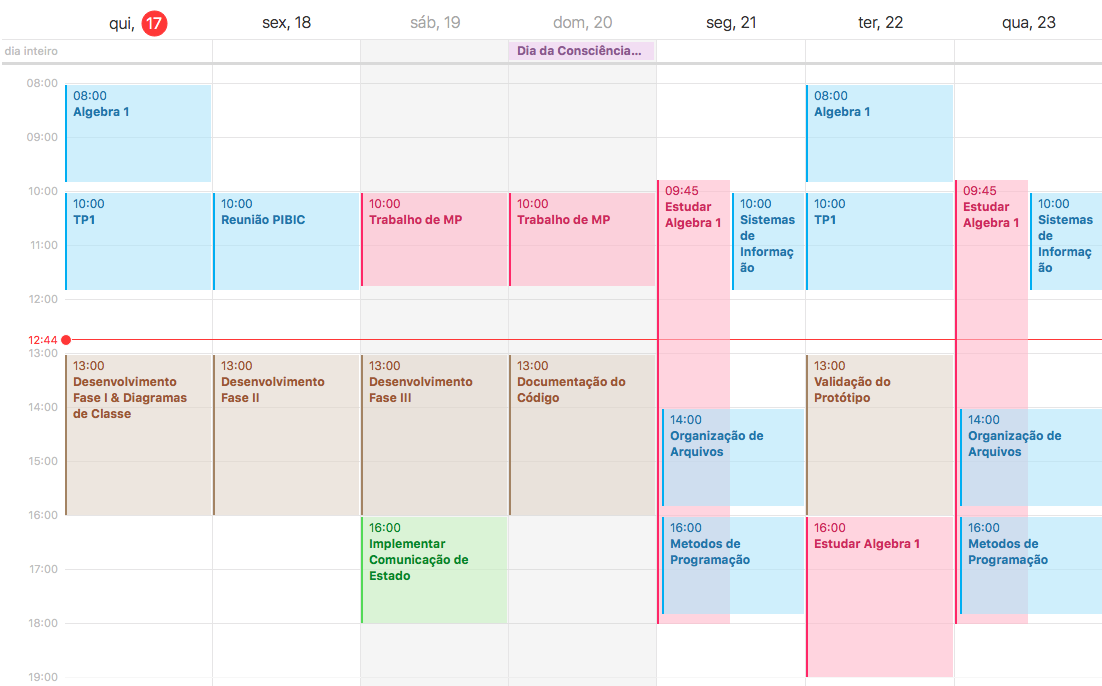
\includegraphics[scale=0.4]{cronograma.png}
		\caption{Cronograma de Execução do Projeto}
	\end{figure}
	
\end{document}
